\section{Kinematics for the Geomagic touch}

As shown on \figref{fig:phantom_omni}, the Phantom omni has 6 joints. The coordinate frame for these joints can be derived as shown on \figref{fig:Frame_phantom}. Note that there is two additional frames for the Phantom omni. These are included because the distance between joint 3 and 4, 5 and 6, can not be defined as frame $O_3$ does not intersect with $x_4$ and $O_5$ does not intersect with $x_6$. This is solved by introducing the two frames upon $O_3$ and $O_5$ in such a way that the frames are rotated, thus fulfilling the DH(1) and DH(2) rule and thereby enabling the opportunity of defining the distance. \\
The \gls{DH} parameters can then be derived as shown in \tabref{tab:kin_geo}, where the two additional frames are displayed with roman numbers.

\todo{erase extra frame and edit kinematic chapter. The frame can be added away from the rotating joint, thus simplifes the kinematics parameters.}

\begin{figure}[H]
\centering
\begin{minipage}[H]{.65\textwidth}
\centering
\vspace{0pt}
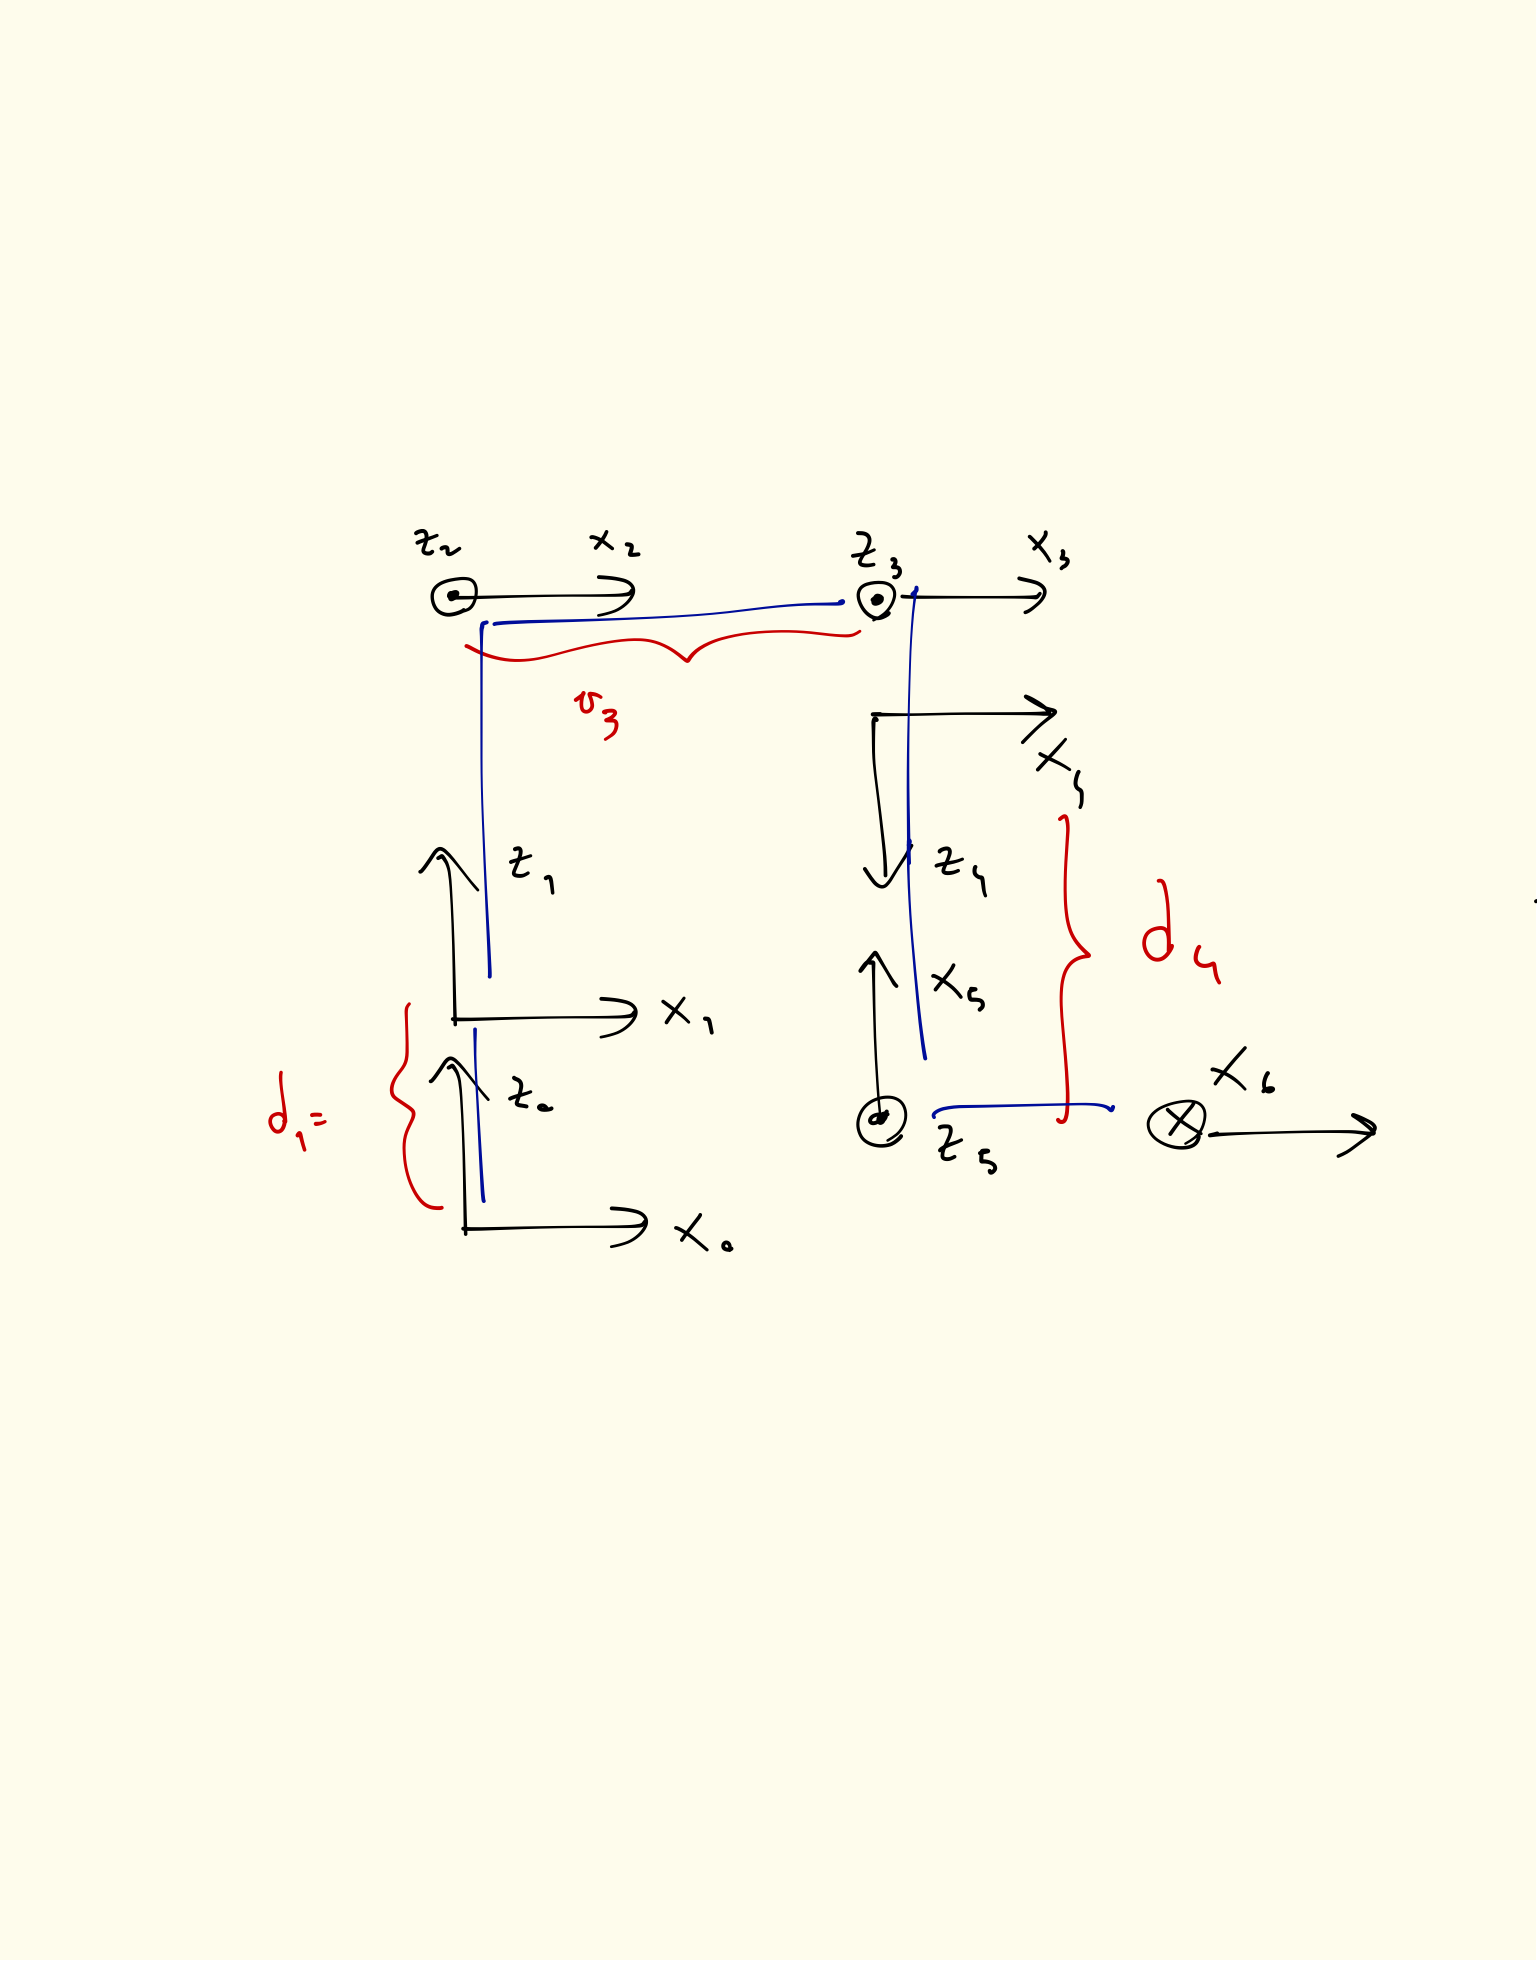
\includegraphics[width=\textwidth]{Geomagic_dh.png}
\caption{Phantom omnis coordinate frames}
\label{fig:Frame_phantom}
\end{minipage}\hfill
\begin{minipage}[H]{.35\textwidth}
\centering
\vspace{95pt}
\begin{tabular}{|l|l|l|l|l|}
\hline
 $j_i$ 	  & $a_i$    & $d_i$ & $\alpha_i$ 		 & $\theta_i$ 			 \\ \hline
 1  	  &  $0$     & $d_1$ & $0$	 & $q_1$ 			     \\ \hline
 2  	  &  $0$   & $0$ 	 & $\frac{\pi}{2}$ 		 		 & $q_2 + \theta_1$ 	 \\ \hline
 3  	  &  $a_3$	 & $0$ & $0$ 		 		 & $q_3$ 					 \\ \hline
 4  	  &  $0$	 & $d_4$ & $\frac{\pi}{2}$ 	 & $q_4$ 			 \\ \hline
 5  	  &  $0$	 & $0$ & $-\frac{\pi}{2}$ 		 		 & $-\frac{\pi}{2} + q_5$ 	 				 \\ \hline
 6  	  &  $0$	 & $0$ & $-\frac{\pi}{2}$ 		 & $\frac{\pi}{2}+q_6$ 				 \\ \hline
\end{tabular}
\vspace{0pt}
\caption{This is the caption for table}
\label{tab:kin_geo}
\end{minipage}
\end{figure}
\todo{Find solution to caption figure/table problem!}







% \begin{figure}[H]
% 	\centering
% 	\begin{subfigure}{.49\textwidth}
% 		\centering
% 		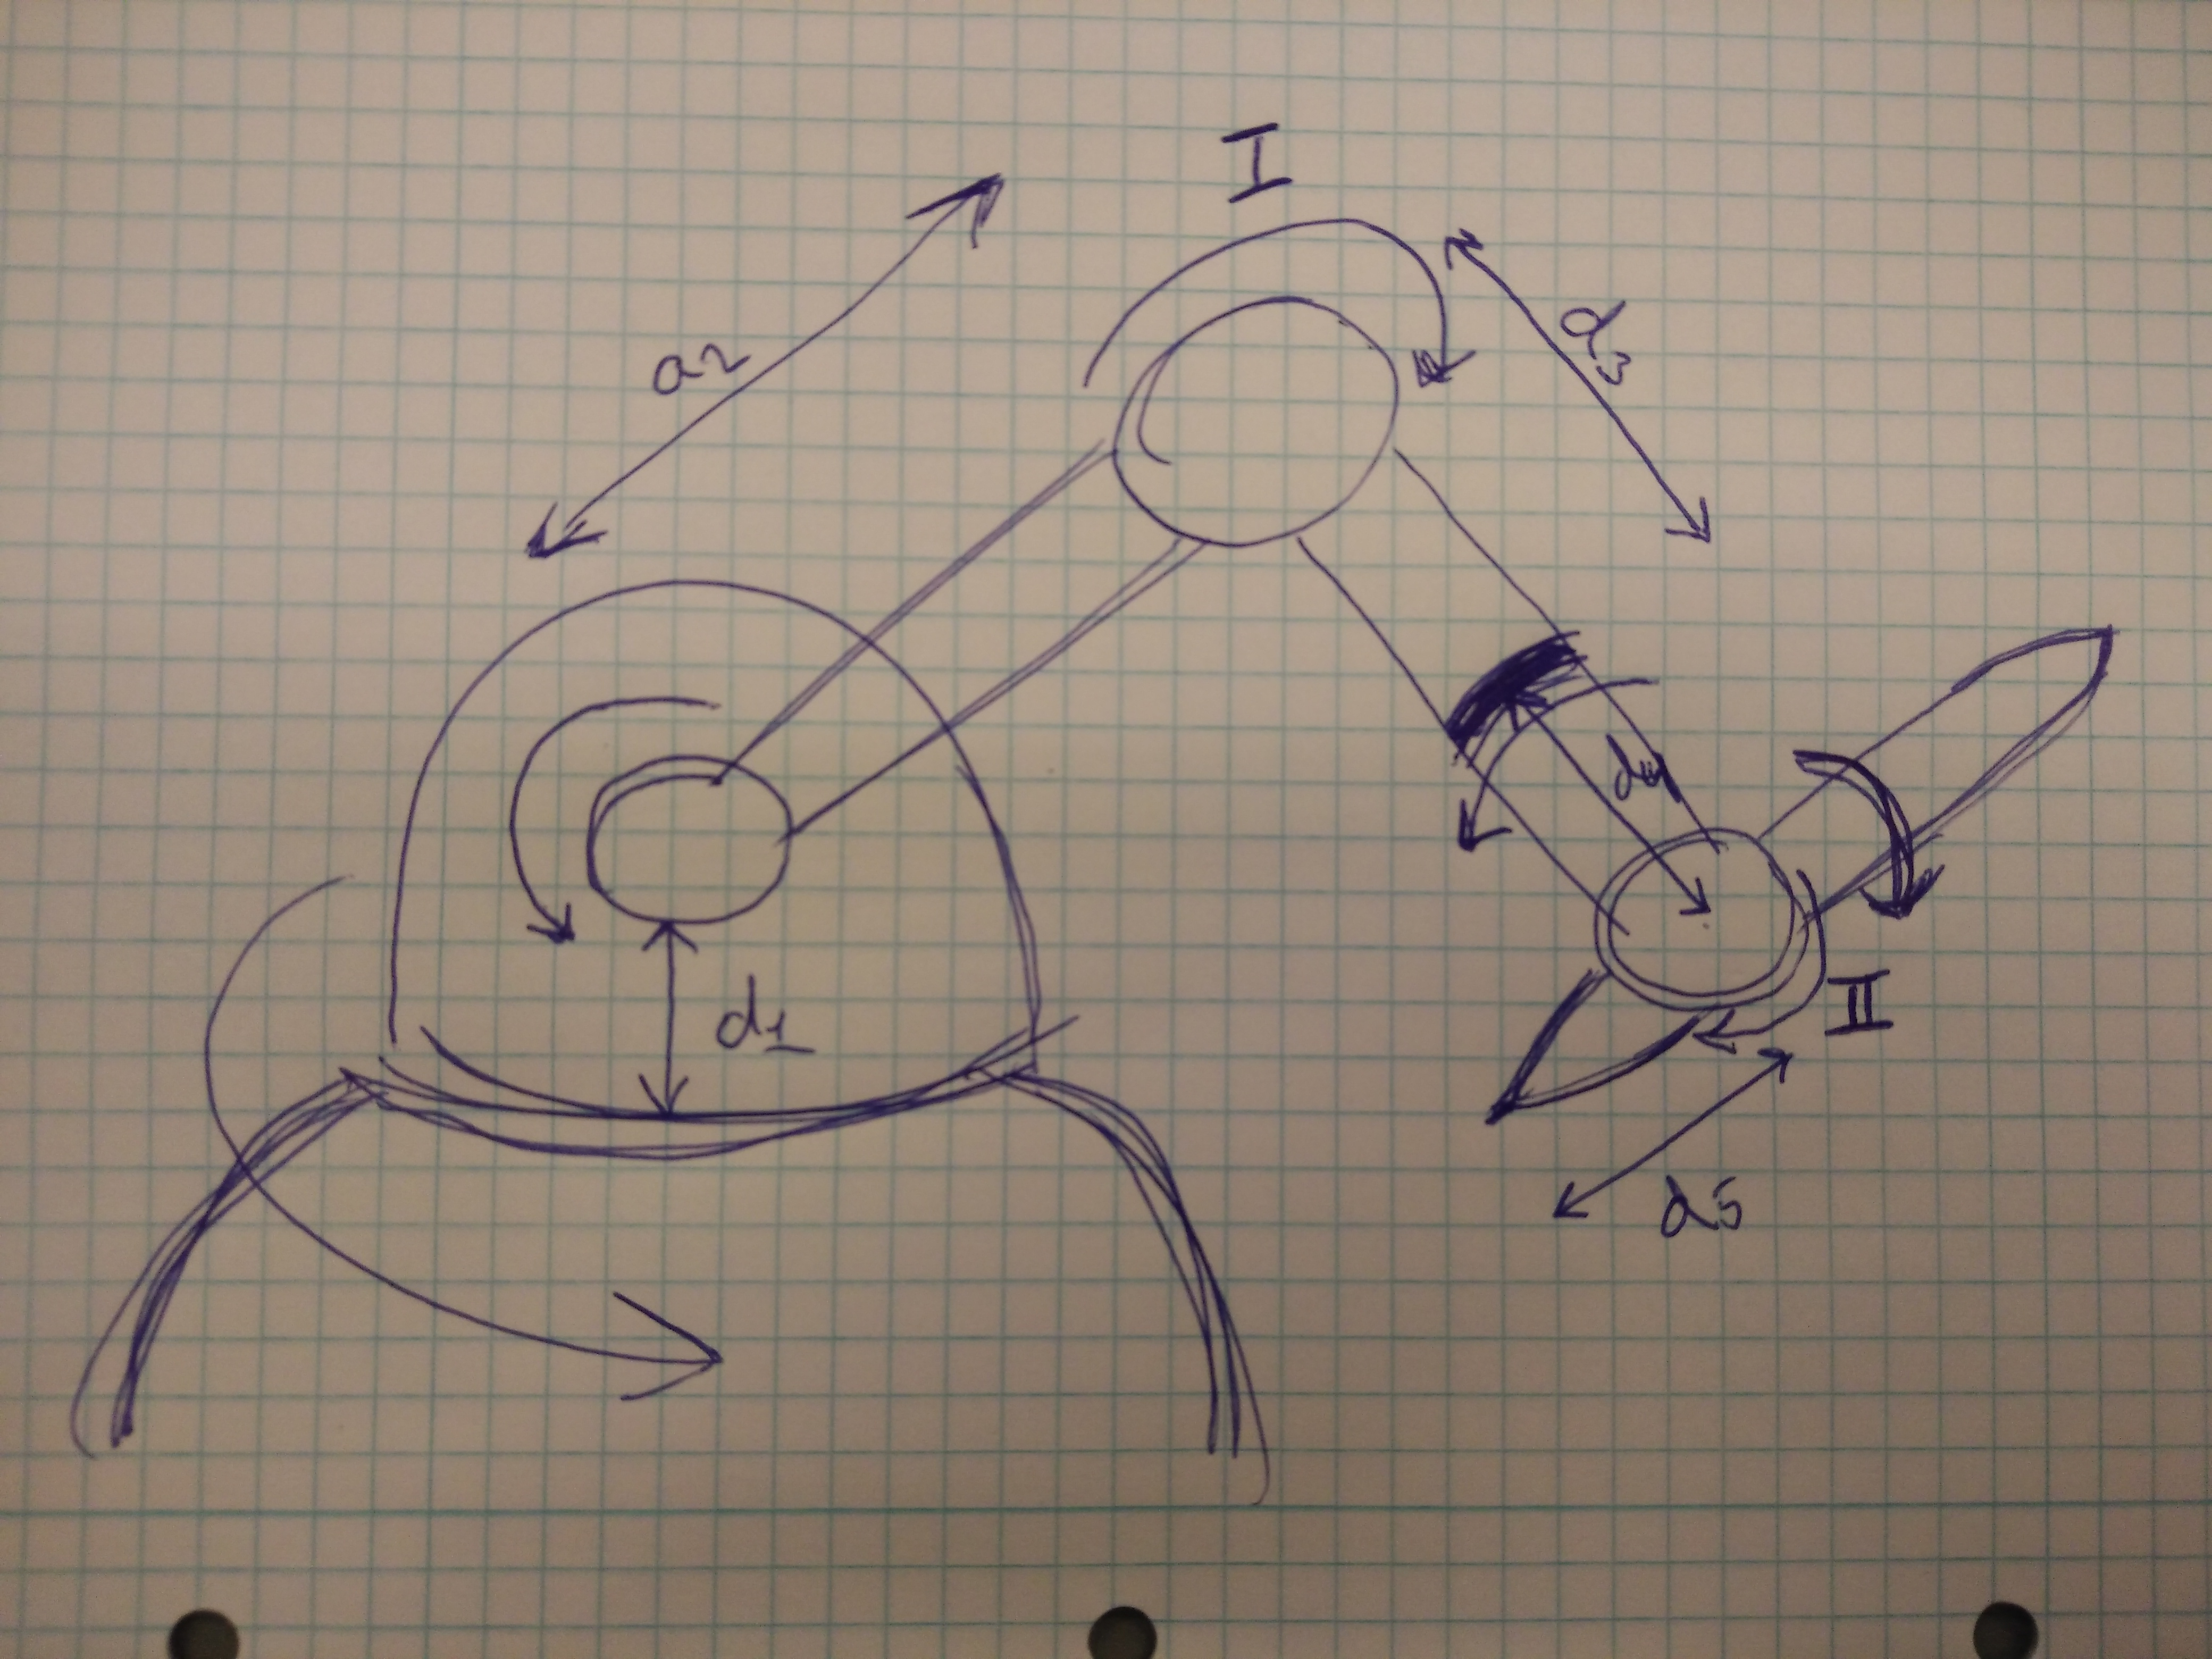
\includegraphics[width=\linewidth]{Fast_draw_Kino.jpg}
% 		\caption{Geomagic touch with all rotational joints and their \gls{DH} parameters.}
% 		\label{fig:1}
% 	\end{subfigure}
% 	\begin{subfigure}{.49\textwidth}
% 		\centering
% 		\includegraphics[width=\linewidth]{Fast_draw_kino2.jpg}
% 		\caption{Frame coordinate system for the Geomagic touch to the deviation of the kinematics.}
% 		\label{fig:Endo_plates}
% 	\end{subfigure}
% \caption{Shows joints positions, the different \gls{DH} parameters and the coordinate frame for each joint. The base frame is difined as $O_{0}$.}
% \label{fig:2}
% \end{figure}


% \begin{table}[H]
% \centering
% \begin{tabular}{|l|l|l|l|l|}
% \hline
%  $j_i$ 	  & $a_i$    & $d_i$ & $\alpha_i$ 		 & $\theta_i$ 			 \\ \hline
%  1  	  &  $0$     & $d_1$ & $\frac{\pi}{2}$	 & $q_1$ 			     \\ \hline
%  2  	  &  $a_2$   & $0$ 	 & $0$ 		 		 & $q_2 + \theta_1$ 	 \\ \hline
%  \rom{1}  &  $0$	 & $0$ 	 & $\frac{\pi}{2}$ 	 & $\frac{\pi}{2} + q_3$ \\ \hline
%  3  	  &  $0$	 & $d_3$ & $0$ 		 		 & $0$ 					 \\ \hline
%  4  	  &  $0$	 & $d_4$ & $\frac{\pi}{2}$ 	 & $\pi + q_4$ 			 \\ \hline
%  \rom{2}  &  $0$	 & $0$ 	 & $\frac{\pi}{2}$   & $\pi +q_5$ 			 \\ \hline
%  5  	  &  $0$	 & $d_5$ & $0$ 		 		 & $0$ 	 				 \\ \hline
%  %6  	  &  $0$	 & $d_6$ & $\theta$ 		 & $q_6$ 				 \\ \hline
% \end{tabular}
% \caption{Tabular which contain the kinematics for the Geomagic touch described in \secref{sec:geo_magic}.The Roman numbers defines the fictional joints}
% \label{tab:kin_geo}
% \end{table}